\section{Introduction}
\label{sec:introduction}

Linguistic steganography hides a secret inside ordinary text.
Early methods mostly swapped synonyms \cite{qiang2023natural}.
Natural language has little spare room, so even small statistical quirks can give a detector something to grab \cite{yang2020vae,kaptchuk2021meteor,Wang_2023}.
Large language models changed the cover: instead of editing an existing sentence, many systems now generate the text \cite{li2023rewriting,lin2024zero,wu2024generative}.
Those systems usually hide bits by steering next-token sampling, which can look fluent while still sitting on a modified distribution.

However, existing LLM-based steganographic systems remain constrained by a fundamental trade-off between statistical security and perceptual naturalness \cite{lin2024zero,wu2024generative,li2023rewriting}. While a model may output grammatically and statistically fluent sentences, these often lack the deep semantic coherence required for specific communicative contexts, such as threaded social media discussions \cite{liao2024co,wang2023hi,zhang2024controllable}. A comment that is fluent but off-topic is conspicuous to a human reader and to a semantic checker.

We hide the payload in two conversational choices rather than in token probabilities.
Bits select (i) which comment to reply to in a depth-first flattened thread, and (ii) which \textit{Angle} to talk about from a list both parties rebuild from the public thread and a shared research procedure.
A language model then writes an ordinary visible reply for that pair.
We do not use invisible characters.
Before the comment is kept, the sender runs the same Angle decoder the receiver will use and retries if that decode misses.
Figure~\ref{fig:token-vs-intent} contrasts token-level embedding with this two-layer selection channel.
% ------------------------------------------------------------------
% AI IMAGE PROMPT (fig:token-vs-intent) -> figures/token_vs_intent_embedding.(png|pdf)
% ------------------------------------------------------------------
% GLOBAL STYLE: Academic technical diagram, flat vector infographic, 16:9 or 2:1 landscape,
%   300 DPI target, white or #F8FAFC background, high contrast, sans-serif labels (simulate
%   Helvetica / Inter), slate blue #334155 primary, teal #0D9488 secondary, amber #D97706
%   accents, thin 1--2pt strokes, optional subtle card shadows. No photorealistic humans,
%   no Reddit Snoo or brand logos, no watermarks, no 3D renders, no cluttered stock icons.
% COMPOSITION: Three-column layout. Vertical divider lines or generous whitespace between
%   columns. Top centered small title: "Embedding domain: token vs communicative intent".
% LEFT PANEL (width ~38%): Header bar "Token / distribution embedding (typical)".
%   Below: horizontal row of 8--12 small rectangles as fake tokens (single letters or
%   [tok] placeholders). Arrow down to a stacked bar or histogram labeled "next-token
%   distribution / logits". Second arrow to a die or branching arrows labeled "sampling".
%   Small triangular warning badge with text "often needs white-box logits" and sublabel
%   "fragile in threaded social context". Use cool gray tones; keep diagram busy but legible.
% CENTER (~12%): Large vertical double chevron or bold arrow pointing upward, label
%   "shift to semantic layer" on two lines, color teal.
% RIGHT PANEL (~38%): Header "Semantic / intent embedding (this work)". Generic forum UI:
%   rounded rectangle "Original post" at top; 2--3 nested "Comment" cards with indent guides;
%   one comment node outlined in amber with pin icon, label "Layer 1: reply target".
%   From that node, fan out 4--6 small rounded chips labeled "Angle 0..N" (Layer 2).
%   One chip highlighted; arrow to final speech bubble "Stego reply (cover text)".
%   Optional tiny caption strip: "Shared deterministic reconstruction (thread + research)".
% LEGIBILITY: All English labels at least 8pt equivalent when scaled to single-column
%   figure width in ACM manuscript. Avoid micro-font paragraphs; use short phrases only.
% NEGATIVE PROMPT: blurry text, illegible handwriting, isometric clutter, cyberpunk neon,
%   anime, screenshots of real apps, dense equations, more than two sentences of body text.
% ------------------------------------------------------------------

\begin{figure}[t]
	\centering
	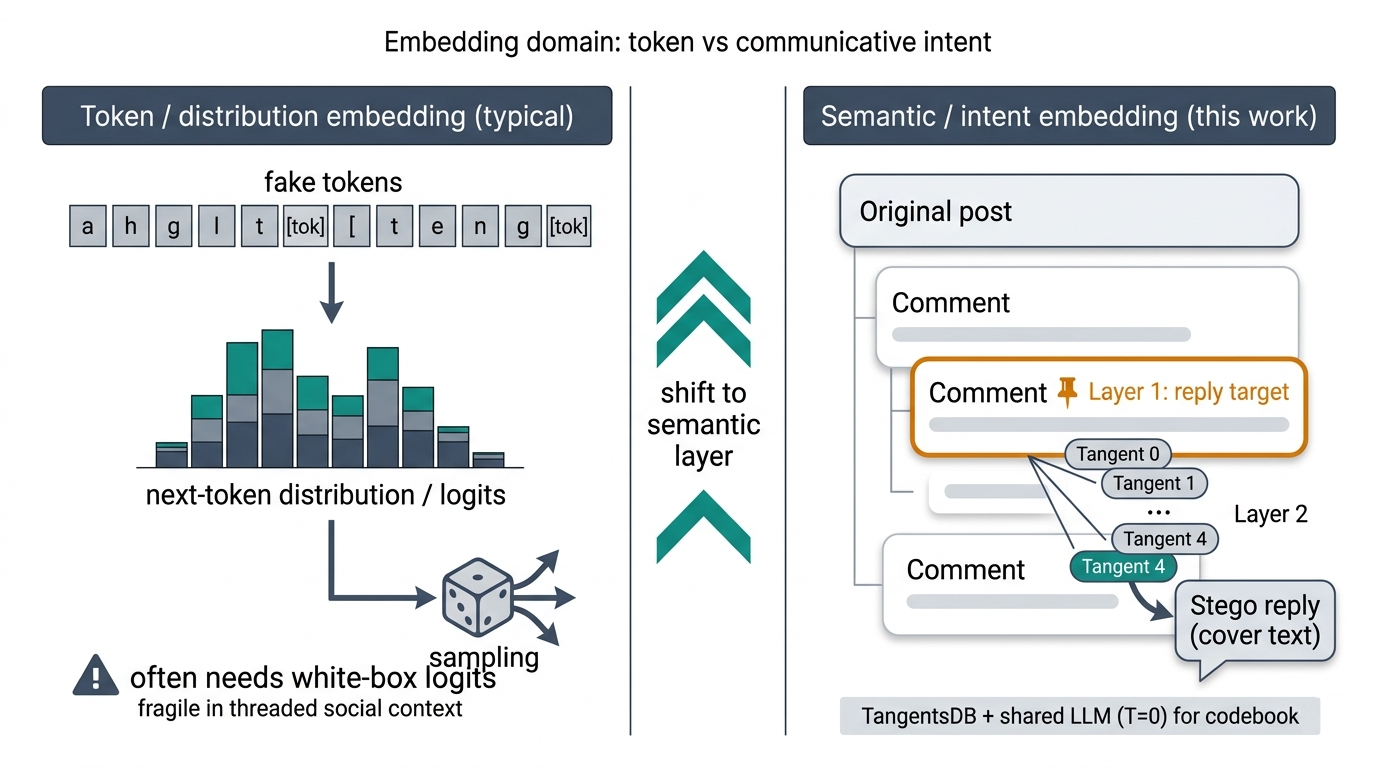
\includegraphics[width=0.78\linewidth]{figures/token_vs_intent_embedding}
	\Description{Side-by-side contrast: token-level steganography versus two-layer semantic embedding (reply placement and thematic intent) in a discussion thread.}
	\caption{Conceptual contrast between token-level embedding and our two-layer semantic embedding over a threaded discussion.}
	\label{fig:token-vs-intent}
\end{figure}

The primary contributions of this paper are:
\begin{itemize}
    \item A two-layer, selection-channel embedding architecture for threaded discussions that encodes bits into reply targeting and Angle selection, with a visible reply rather than a hidden carrier.
    \item A reconstruction pipeline (thread plus reproducible research) that does not need white-box logits. Reported payload recovery still uses sender-side audit metadata.
    \item A closed-loop verification mechanism that simulates decoding before the comment is kept and retries synthesis, with an optional revision pass, under stochastic generation.
    \item An independent LLM-judge comparison on 244 unique-output pairs against the official ZLG baseline, reported together with source-run reliability and a historical 304-pair configuration table, with explicit denominators and without a superiority claim.
\end{itemize}
